% ============================================================
%  main.tex  —  English Master Thesis
%  Department of Finance, College of Management
%  National Taiwan University
%  Compile with: xelatex main (run twice for correct TOC/references)
% ============================================================
\documentclass[12pt, a4paper, oneside]{book}

% ── Fonts (XeLaTeX required) ──────────────────────────────────
% English: Times New Roman (if installed); TeX Gyre Termes is the substitute.
% On Mac/Windows with Times New Roman installed, replace with:
%   \setmainfont{Times New Roman}
\usepackage{fontspec}
\setmainfont{TeX Gyre Termes}

% CJK: 標楷體 (Kai).
% On Mac/Windows use: \setCJKmainfont{標楷體}
% On this Linux system AR PL UKai TW is the equivalent.
\usepackage{xeCJK}
\setCJKmainfont{AR PL UKai TW}
\setCJKsansfont{AR PL UKai TW}

% ── Page layout (top 3cm, bottom 2cm, left/right 3cm) ─────────
\usepackage{geometry}
\geometry{a4paper, top=3cm, bottom=2cm, left=3cm, right=3cm}

% ── Line spacing: double ──────────────────────────────────────
\usepackage{setspace}
\doublespacing

% ── Page numbers at bottom centre ────────────────────────────
\pagestyle{plain}

% ── NTU logo watermark (top-right every page) ─────────────────
% ── Shared preamble (tables, math, figures, custom commands) ──
% ============================================================
%  preamble.tex  —  shared by main.tex (English) and main_zh.tex (Chinese)
% ============================================================

% --- Tables --------------------------------------------------
\usepackage{booktabs}       % \toprule \midrule \bottomrule
\usepackage{multirow}       % \multirow{n}{*}{text}
\usepackage{makecell}       % line breaks inside cells
\usepackage{tabularx}       % auto-width columns

% --- Figures -------------------------------------------------
\usepackage{graphicx}
\usepackage{caption}        % \captionof for non-floating tables
\usepackage{subcaption}     % \begin{subfigure}

% --- Math ----------------------------------------------------
\usepackage{amsmath}
% \usepackage{amssymb}
\usepackage{bm}             % bold math \bm{}

% --- Numbers & Units -----------------------------------------
\usepackage{siunitx}
\usepackage{enumitem}
\sisetup{
  round-mode      = places,
  round-precision = 3,
  table-format    = 1.3,
}

% --- Typography ----------------------------------------------
\usepackage{microtype}      % better line breaking

% --- Diagrams ------------------------------------------------
\usepackage{tikz}
\usetikzlibrary{shapes.geometric, arrows.meta, positioning, fit, backgrounds}

% --- Bibliography --------------------------------------------
% natbib provides \citet{} and \citep{}
\usepackage[round,authoryear]{natbib}

% --- Cross-references ----------------------------------------
\usepackage{hyperref}
\usepackage{cleveref}       % \cref{} \Cref{}

% --- Fonts ----------------------------------------
\usepackage{amsfonts}

% ============================================================
%  Terminology Glossary (EN → ZH)
%  Cross-Sectional           橫截面
%  Ranking Loss              排序損失
%  Gradient Accumulation     梯度累積
%  Ensemble                  集成
%  Feature Configuration     特徵組合
%  Walk-forward              滾動前向
%  Sharpe Ratio              夏普比率
%  Long-Short Portfolio      多空投資組合
%  Variable Selection Net    變數選擇網路
%  Gated Residual Network    門控殘差網路
%  Temporal Fusion Transformer  時序融合轉換器
%  Cross-Asset Attention     跨資產注意力
% ============================================================

% --- Custom commands -----------------------------------------
\newcommand{\SR}{\mathrm{SR}}          % Sharpe Ratio abbreviation
\newcommand{\NW}{\mathrm{NW}}          % Newey–West
\newcommand{\btau}{\bm{\tau}}
\newcommand{\bx}{\bm{x}}
\newcommand{\by}{\bm{y}}
\newcommand{\cL}{\mathcal{L}}
\newcommand{\cF}{\mathcal{F}}
\newcommand{\R}{\mathbb{R}}

% Bold table header helper
\renewcommand{\thead}[1]{\textbf{#1}}

% Significance stars
\newcommand{\sig}[1]{%
  \ifnum#1=3 $^{***}$\fi
  \ifnum#1=2 $^{**}$\fi
  \ifnum#1=1 $^{*}$\fi
}



% NTU logo watermark
% NTU watermark following mediaic/NTU_MS_Thesis.
% Source settings: vector NTU seal, absolute scale 40%, opacity 20%,
% behind page, watermark center 2.5 cm from top and right.
\usepackage{eso-pic}

\newcommand{\NTUWatermark}{%
  \AddToShipoutPictureBG{%
    \put(\LenToUnit{\dimexpr\paperwidth-2.5cm-50.4bp\relax},
         \LenToUnit{\dimexpr\paperheight-2.5cm-50.4bp\relax}){%
      \begin{tikzpicture}
        \node[anchor=south west, inner sep=0pt, opacity=0.20]
          {
\includegraphics[width=100.8bp]{NTU_logo_gray}};%
      \end{tikzpicture}%
    }%
  }%
}

\NTUWatermark


% ── hyperref settings (loaded in preamble) ───────────────────
\hypersetup{
  colorlinks = true,
  linkcolor  = black,
  citecolor  = black,
  urlcolor   = black,
}

% ============================================================
\begin{document}

%% ─────────────────────────────────────────────────────────────
%% Front matter (Roman page numbers)
%% ─────────────────────────────────────────────────────────────
\frontmatter

% ── Cover page ───────────────────────────────────────────────
\begin{titlepage}
\begin{singlespace}
\centering
\vspace*{1cm}

{\fontsize{18}{27}\selectfont 國立臺灣大學管理學院財務金融研究所\par
                               碩士論文\par}
{\fontsize{14}{21}\selectfont Department of Finance\par
                               College of Management\par}
{\fontsize{16}{24}\selectfont National Taiwan University\par
                               Master Thesis\par}

\vfill

{\fontsize{18}{27}\selectfont 利用排序正規化深度學習進行\\
                               加密貨幣橫截面報酬預測\par}
\vspace{6pt}
{\fontsize{18}{27}\selectfont Cross-Sectional Cryptocurrency Return Prediction\\
                               via Rank-Normalized Deep Learning\par}

\vfill

{\fontsize{18}{27}\selectfont 陳\quad 芃\par
                               Peng Chen\par}

\vfill

{\fontsize{18}{27}\selectfont 指導教授：蕭湛東 博士\par
                               Advisor: Dr.\ Lawrence Hsiao\par}

\vfill

{\fontsize{18}{27}\selectfont 中華民國 115 年 6 月\par
                               June 2026\par}

\vspace{3cm}
\end{singlespace}
\end{titlepage}

% ── Committee Approval ───────────────────────────────────────
\chapter*{Committee Approval}
\addcontentsline{toc}{chapter}{Committee Approval}
\thispagestyle{plain}

\vspace{1cm}
\noindent This thesis entitled \textit{Cross-Sectional Cryptocurrency Return Prediction via
Rank-Normalized Deep Learning} by Peng Chen (Student ID: R12723071) has been
examined and approved by the following examination committee on
\underline{\hspace{3em}} / \underline{\hspace{3em}} / \underline{\hspace{3em}} (YYYY/MM/DD)
at the Graduate Institute of Finance, National Taiwan University.

\vspace{3cm}
\noindent Examination Committee:

\vspace{1.5cm}
\hspace{4cm}\underline{\hspace{8cm}} (Advisor)

\vspace{1.2cm}
\hspace{4cm}\underline{\hspace{8cm}}

\vspace{1.2cm}
\hspace{4cm}\underline{\hspace{8cm}}

\vspace{1.2cm}
\hspace{4cm}\underline{\hspace{8cm}}

\vspace{2cm}
\noindent Department Chair / Graduate Institute Director\underline{\hspace{5cm}}

% ── Acknowledgments ──────────────────────────────────────────
\chapter*{Acknowledgments}
\addcontentsline{toc}{chapter}{Acknowledgments}
\thispagestyle{plain}

\noindent I am deeply grateful to my advisor, Dr.\ Lawrence Hsiao, for his invaluable
guidance, insightful suggestions, and continuous encouragement throughout this research.

% ── Chinese Abstract ─────────────────────────────────────────
\chapter*{中文摘要}
\addcontentsline{toc}{chapter}{中文摘要}
\thispagestyle{plain}

\begin{singlespace}
% 對應英文：sections/01_abstract.tex
% TODO: 翻譯後請同步更新英文版的修改

預測下週哪些加密貨幣將超越同類資產，本質上是一個橫截面排序問題，
然而過去的研究普遍採用不適合排序目標的時間序列損失函數。
本文證明，這種目標函數與評估標準之間的不匹配，
是深度學習模型在此類任務中表現遜於普通最小二乘法（OLS）的主要原因。

本文的核心方法貢獻，在於將 ListNet 排序損失的目標訊號從原始報酬替換為
橫截面排名百分位：每個資產依其在當週橫截面中的排名，被賦予介於 $[0, 1]$
的監督信號（Poh 等人，2021），無論當週報酬的絕對波動幅度為何，
每個資產對損失梯度的貢獻均等。

本文在一個涵蓋 324 週 $\times$ 86 種加密貨幣的週資料面板上，
評估三種深度學習架構——具有跨資產注意力的 LSTM、採用完整變數選擇網路的時序融合轉換器（TFT），
以及全新設計的橫截面門控網路（CS-Gated）——並與六種傳統基準模型進行比較。

最佳模型 CS-Gated（以鏈上特徵訓練）在年化夏普比率上達到 2.75（等權多空組合），
而 LSTM 搭配川普社群媒體與 ETF 資金流特徵則達到 2.13。
整體結果顯示，深度學習在正確的排序損失下可與傳統方法競爭，
但不同模型對不同訊號型態各有優勢，隨機森林在高維資訊集下仍具強勁表現。
消融研究（ablation study）確認，排名正規化搭配梯度累積，
是促成績效改善的關鍵機制。

\end{singlespace}

\vspace{1em}
\noindent\textbf{關鍵詞：}加密貨幣、橫截面預測、排序損失、時序融合轉換器、機器學習

% ── English Abstract ─────────────────────────────────────────
\chapter*{Abstract}
\addcontentsline{toc}{chapter}{Abstract}
\thispagestyle{plain}

Predicting which cryptocurrencies will outperform in the following week
is fundamentally a cross-sectional ranking task, yet prior work has
applied time-series loss functions ill-suited to ranking objectives.
We demonstrate that this mismatch is the primary reason deep learning
models often underperform ordinary least squares in standard configurations.
%
Our key methodological contribution is the use of rank-percentile
normalized targets with ListNet ranking loss: instead of softmax-weighting
raw returns, we assign each asset its cross-sectional rank percentile as
the supervision signal, eliminating scale sensitivity across heterogeneous
volatility regimes.
%
We evaluate three deep learning architectures—LSTM with cross-asset
attention, a corrected Temporal Fusion Transformer (TFT), and a novel
CrossSectionalGatedNet (CS-Gated)—against six traditional baselines on
a panel of 324 weeks $\times$ 86 cryptocurrencies.
%
The best model, CS-Gated trained on on-chain features, achieves an
annualized Sharpe ratio of 2.75 (equal-weight long-short portfolio),
while LSTM with Trump social media and ETF flow features reaches 2.13.
The results show that deep learning becomes competitive once the ranking
objective is specified correctly, although different architectures remain
best suited to different signal types.
An ablation study confirms that rank normalization together with gradient
accumulation, rather than architectural novelty alone, drives the improvement.


\vspace{1em}
\noindent\textbf{Keywords:} cryptocurrency, cross-sectional prediction, ranking loss,
temporal fusion transformer, machine learning

% ── Table of Contents, List of Figures, List of Tables ───────
\tableofcontents
\listoffigures
\listoftables

%% ─────────────────────────────────────────────────────────────
%% Main text (Arabic page numbers)
%% ─────────────────────────────────────────────────────────────
\mainmatter

\chapter{Introduction}
\label{sec:intro}
The cryptocurrency market has grown from a single asset—Bitcoin, introduced by
\citet{nakamoto2008bitcoin} as a decentralized peer-to-peer payment system—into
a diverse asset class encompassing thousands of tokens with heterogeneous
on-chain economics, governance structures, and macro exposures.
\citet{liu2022cryptocurrency} document that the cross-section of cryptocurrency
returns exhibits its own set of risk factors, including momentum and size premia
that are structurally distinct from their equity counterparts.
With over 86 actively traded tokens spanning divergent network fundamentals
and social sentiment signals, predicting which assets will outperform their peers
in the following week is a natural cross-sectional learning problem—one that
demands models capable of synthesizing heterogeneous feature sets while learning
a \emph{relative}, rather than absolute, notion of return.

\paragraph{Prior work and the research gap.}
The foundational study of \citet{gu2020empirical} demonstrates that machine
learning models—in particular, tree ensembles and deep networks—substantially
outperform linear baselines for cross-sectional equity return prediction when
feature sets are rich and model capacity is appropriately regularized.
\citet{freyberger2020dissecting} extend this finding to a nonparametric
setting, showing that nonlinear interactions among stock characteristics carry
significant incremental predictive power.
Applying these insights to cryptocurrency markets is appealing in principle
but nontrivial in practice.
The primary obstacle is \emph{cross-sectional volatility heterogeneity}: a
Bitcoin weekly return might span $\pm 5\%$ while a small-cap altcoin regularly
moves $\pm 30\%$.
When the standard ListNet loss \citep{cao2007learning} is trained with raw
weekly returns as softmax targets, the resulting target distribution $Q$ is
dominated in volatile weeks by a handful of extreme-return assets, and nearly
uniform in calm weeks.
This instability produces high-variance gradient estimates that undermine
consistent ranking performance across market regimes.
\citet{poh2021building} identify this failure mode in equity cross-sectional
strategies and propose replacing raw-return targets with cross-sectional rank
percentiles; we adopt and extend their framework to the cryptocurrency setting,
where the problem is more acute due to the larger cross-sectional dispersion
in volatility.

On the data side, \citet{liu2022cryptocurrency} and \citet{cong2021tokenomics}
establish that on-chain network metrics—such as network value-to-transaction
ratio (NVT) and market-value-to-realized-value (MVRV)—contain information
about the fundamental valuation state of individual tokens that is orthogonal
to price-based momentum signals.
Beyond on-chain data, the role of alternative information sources in asset
pricing has been well established in the equity literature.
\citet{tetlock2007giving} demonstrates that media pessimism predicts short-run
downward price pressure in equity markets, and \citet{bollen2011twitter}
show that Twitter-derived mood measures Granger-cause changes in the Dow Jones
Industrial Average.
We extend this line of inquiry to a novel source: the social media activity of
a single, highly influential policy actor (the 45th and 47th U.S.\ President),
whose public communications on cryptocurrency regulation and macroeconomic
tariff policy have preceded market-wide repricing events.
A further structural data source—unavailable before January 2024—is the
granular daily flow data for spot Bitcoin and Ethereum exchange-traded funds
published by Farside Investors
\citep{bitcoin_etf_farside,ethereum_etf_farside}, which permits decomposition of ETF
inflows into net new capital and legacy-holder rotations.
To the best of our knowledge, this paper is the first to integrate on-chain fundamentals,
policy-linked social media signals, and ETF structural flows into a unified
cross-sectional ranking framework evaluated on a live 86-token universe.

\paragraph{Architecture considerations.}
Two families of temporal deep learning architectures are well suited to
sequential financial data.
The Long Short-Term Memory network \citep{hochreiter1997long} encodes the
$L$-step feature history into a fixed-size hidden state via gated recurrence,
and has remained a competitive baseline for financial time series despite the
rise of attention-based models.
The Temporal Fusion Transformer \citep{lim2021temporal} combines interpretable
Variable Selection Networks (VSN) with multi-head self-attention
\citep{vaswani2017attention}, enabling explicit feature selection at each
time step and scalable handling of heterogeneous input types.
However, \citet{gu2020empirical} also observe that cross-sectional features
can dominate temporal features for equity ranking—motivating a purely
cross-sectional architecture that operates on contemporaneous inputs alone,
without any temporal encoder.
We formalize and test this design hypothesis through our CrossSectionalGatedNet.

\paragraph{Contributions.}
Building on the above foundation, this paper makes four targeted contributions
to the cross-sectional cryptocurrency prediction literature:
\begin{enumerate}
  \item \textbf{Rank-normalized ListNet targets.}
        Following \citet{poh2021building}, we replace raw returns with
        cross-sectional rank percentiles $\in [0,1]$ as softmax targets,
        ensuring equal contribution of each asset regardless of its
        absolute volatility and stabilizing the cross-entropy gradient
        across heterogeneous market regimes.
  \item \textbf{Gradient accumulation.}
        The effective cross-sectional batch size is increased from 86
        (one week's cross-section) to $86 \times 4 = 344$ assets per
        gradient step, providing a more stable rank estimate for the
        ListNet loss and reducing stochasticity in the gradient direction.
  \item \textbf{CrossSectionalGatedNet.}
        A new architecture consisting purely of Gated Residual Networks
        (GRN) and cross-asset attention, with no temporal encoder.
        Motivated by \citet{gu2020empirical}, we test whether the
        cross-sectional structure alone—without temporal modeling—is
        sufficient for the ranking task when on-chain fundamentals
        dominate the predictive signal.
  \item \textbf{Full-scale TFT Variable Selection Network.}
        We implement a per-variable shared GRN ($\sim$27K parameters) for
        nonlinear variable selection, closer to the original
        \citet{lim2021temporal} specification, and show that this design
        substantially stabilizes feature selection.
\end{enumerate}

\paragraph{Paper organization.}
\Cref{sec:related} reviews related work in greater detail.
\Cref{sec:data} describes the 86-token, 324-week balanced panel and its
seven feature groups.
\Cref{sec:method} formalizes the ranking loss and the four model architectures.
\Cref{sec:experiments} details the training setup, six feature configurations,
and 32-seed ensemble strategy.
\Cref{sec:results} presents the main cross-model comparison.
\Cref{sec:analysis} provides ablation studies, Granger causality tests,
transaction cost sensitivity analysis, and sub-period robustness checks.
\Cref{sec:conclusion} concludes.


\chapter{Related Work}
\label{sec:related}
\section{Machine Learning for Cross-Sectional Returns}

\citet{gu2020empirical} provide the canonical empirical benchmark for
machine-learning-based cross-sectional asset pricing.
Using a large equity-characteristic panel, they show that tree ensembles
and neural networks outperform linear baselines when feature sets are rich
and model capacity is regularized appropriately.
\citet{freyberger2020dissecting} reinforce this conclusion from a
nonparametric perspective, demonstrating that the incremental predictive
power of asset characteristics often lies in nonlinear interactions rather
than in any single characteristic taken in isolation.
Viewed jointly, this literature suggests that the central modeling problem
in cross-sectional return prediction is not merely temporal extrapolation,
but the extraction of structured relative information from a heterogeneous
feature set.

The cryptocurrency literature confirms that the asset class is predictable,
but it is less settled on how much model complexity is actually useful.
\citet{liu2022cryptocurrency} establish the basic risk-factor structure of
cryptocurrency returns, documenting momentum and size premia that resemble
equity analogues only superficially.
More directly related to our setting, \citet{cakici2022crypto_ml} show that
machine-learning models can generate economically meaningful gains in the
cross-section of cryptocurrency returns, although the incremental benefit of
very high model complexity is limited.
\citet{filippou2024crypto_ml} reach a complementary conclusion: with a rich
set of network, momentum, technical, and attention variables, nonlinear
methods deliver substantial out-of-sample predictive and economic value.
These studies jointly suggest that the key question is not whether
cryptocurrency returns are predictable, but how the learning problem should
be formulated so that heterogeneous predictors can be turned into a stable
cross-sectional ranking.

\section{Learning to Rank in Finance}

The learning-to-rank literature \citep{cao2007learning} offers a natural
foundation for long-short portfolio formation because the investment problem
is inherently ordinal: the objective is to place assets in the correct
relative order, not necessarily to forecast their exact subsequent return.
\citet{poh2021building} provide the closest precursor to our approach.
They show that standard ListNet training becomes unstable when raw returns
are used directly as softmax targets, because target sharpness varies across
weeks with the cross-sectional dispersion of returns.
Replacing raw-return targets with cross-sectional rank percentiles produces
substantially more stable long-short performance in equities.

Our contribution builds directly on this insight, but in a setting where the
problem is arguably more severe.
Cross-sectional volatility heterogeneity is considerably larger in
cryptocurrency markets than in equities, so any objective that depends on
raw-return scale is more prone to unstable gradients.
We therefore adopt the rank-percentile ListNet target and complement it with
gradient accumulation, treating stable objective design as a first-order
methodological requirement rather than a minor training detail.

\section{Temporal Deep Learning Architectures}

Long Short-Term Memory networks \citep{hochreiter1997long,fischer2018lstm_finance}
remain a strong baseline for financial sequence modeling because they can
extract local temporal dependence with relatively controlled parameter count.
This is especially relevant when predictors exhibit short-lived persistence,
as in event-driven social media activity or ETF flow sequences.

The Temporal Fusion Transformer \citep{lim2021temporal} extends this design
space by combining recurrent encoding, Variable Selection Networks (VSN),
and attention-based temporal aggregation.
Relative to generic Transformer architectures \citep{vaswani2017attention},
TFT is particularly attractive for financial panels with heterogeneous
predictors because it provides an explicit mechanism for feature selection
and interpretability.
At the same time, its larger capacity also makes it more vulnerable to
training instability when the effective sample size is limited.
This trade-off is one motivation for our side-by-side comparison of LSTM,
TFT, and a purely cross-sectional architecture.

\section{Alternative Data Sources}

The use of alternative data in financial prediction is now well established.
\citet{tetlock2007giving} show that media tone predicts short-horizon stock
returns, while \citet{bollen2011twitter} document predictive content in
Twitter-derived mood measures.
In the cryptocurrency setting, \citet{maitre2025social} provide more direct
evidence that social-media-based attention is related to the cross-section of
crypto returns.
These studies collectively motivate the use of text-derived or attention-like
signals as complements to price and fundamental information.

Our Trump social media variables differ from general sentiment proxies in an
important respect: they are designed to capture policy-linked signals from a
single high-impact political actor rather than diffuse market mood.
This makes them structurally closer to event variables than to broad
attention measures.

ETF flow data provides a second form of alternative information that is
distinct from both prices and on-chain activity.
Since the approval of spot Bitcoin ETFs in January 2024, the daily flow data
published by Farside Investors
\citep{bitcoin_etf_farside,ethereum_etf_farside} has made it possible to separate
legacy-holder rotations out of Grayscale products from genuinely new capital
entering the asset class.
That decomposition is economically meaningful because it distinguishes
supply-side pressure from demand-side expansion, and is therefore a
potentially useful predictor of cross-sectional dispersion even if it is not
always informative about market direction.

\section{Statistical Inference}

Evaluating financial machine-learning strategies requires inference tools
that remain valid under serial dependence and non-normal return
distributions.
We therefore use Newey--West heteroskedasticity and autocorrelation
consistent statistics \citep{newey1987simple,newey1994automatic} and the
stationary bootstrap of \citet{politis1994stationary}.
These methods do not improve predictive performance, but they reduce the
risk of mistaking concentrated short-sample performance for robust evidence,
which is particularly important given the 49-week test window in this study.


\chapter{Data}
\label{sec:data}
\section{Panel Overview}

The empirical analysis uses the replication package supplied with this
thesis rather than re-downloading every raw input from its original upstream
provider.
The base file, \path{crypto_panel_features.npz}, is a processed weekly
cryptocurrency panel with $T = 324$ calendar weeks
(2020-01-05 to 2026-03-15), $N = 86$ tickers, one next-week return target,
and 49 pre-existing predictor columns.
The augmented file, \path{crypto_panel_features_with_etf.npz}, appends
four granular ETF-flow variables, so the final research panel has 53
predictor columns.
The six information sets used in the empirical comparisons draw on a
42-feature subset of those columns.

The base panel is treated as a processed input because the current repository
does not contain enough raw-vendor metadata to reconstruct every original
source for the 49 pre-existing variables.
For that reason, the data discussion below separates directly observable
replication files from upstream provenance that is not recoverable from the
files provided.
This is a deliberate reporting constraint: feature names and transformations
are reported when they can be inspected in the files and code, but external
vendors are not attributed unless the repository or an official source
supports the attribution.

Missing values are encoded as $-99.99$ and masked in both loss computation
and portfolio evaluation.
The fixed 86-token universe is therefore best interpreted as the asset
universe encoded in the replication package, not as a fully auditable
historical listing universe.

\section{Observed Data Files and Provenance}

\Cref{tab:data_provenance} lists the data files that can be directly verified
in the replication package.
Only the two Farside CSV files are raw external downloads visible in the
repository.
The NPZ files are processed research inputs or saved benchmark arrays.

\begin{table}[t]
\centering
\caption{Directly observed data files in the replication package.}
\label{tab:data_provenance}
\scriptsize
\begin{tabularx}{\linewidth}{>{\raggedright\arraybackslash}p{0.20\linewidth}X >{\raggedright\arraybackslash}p{0.16\linewidth}X >{\raggedright\arraybackslash}p{0.12\linewidth}}
\toprule
\thead{File} & \thead{Variables / role} & \thead{Period} &
\thead{Construction step} & \thead{Raw source observable?} \\
\midrule
\path{crypto_panel_features.npz}
  & Processed base panel: dates, tickers, next-week returns, and 49
    pre-existing predictors.
  & Weekly, 2020-01-05--2026-03-15
  & Loaded as the pre-existing base panel; no raw-source reconstruction is
    possible from the current files.
  & No \\
\path{crypto_panel_features_with_etf.npz}
  & Final v6 panel after appending four Farside ETF variables.
  & Weekly, 2020-01-05--2026-03-15
  & Constructed by augmenting the base panel with weekly GBTC, BTC ex-GBTC,
    ETHE, and ETH ex-ETHE flow variables.
  & Partly \\
\path{market_cap.npz}
  & Saved market-cap matrix used for market benchmark construction.
  & Weekly, 2020-01-05--2026-03-15
  & Loaded as an aligned matrix for weighting and benchmark calculations.
  & No \\
\path{farside_btc.csv}
  & Daily U.S. spot Bitcoin ETF flow table, including GBTC and total flows.
  & Daily rows, 2024-01-11--2026-03-06
  & Parsed from CSV, converted to signed values, then aggregated to weekly
    GBTC and BTC ex-GBTC flows.
  & Yes \\
\path{farside_eth.csv}
  & Daily U.S. spot Ethereum ETF flow table, including ETHE and total flows.
  & Daily rows, 2024-07-23--2026-03-06
  & Parsed from CSV, converted to signed values, then aggregated to weekly
    ETHE and ETH ex-ETHE flows.
  & Yes \\
\bottomrule
\end{tabularx}
\end{table}

The Farside files correspond to the Bitcoin and Ethereum ETF flow tables
published by Farside Investors \citep{bitcoin_etf_farside,ethereum_etf_farside}.
In the CSV format, parenthesized values denote outflows and are parsed as
negative numbers, dashes are treated as missing or zero-flow cells depending
on the aggregation step, and daily rows are aggregated to the weekly panel
calendar.
For each week, flows in the interval from the previous panel date to the
current panel date are summed.
The four appended variables are GBTC flow, total Bitcoin ETF flow excluding
GBTC, ETHE flow, and total Ethereum ETF flow excluding ETHE.
Each weekly series is then transformed with the same 52-week rolling
z-score rule used for other time-series predictors.

\section{Feature Categories}

\Cref{tab:features} summarizes the 42 features actually used in the model
comparisons.
The table reports variable groups and examples; it should not be read as a
claim about raw upstream vendors for the pre-existing base-panel variables.
The grouping reflects the main conceptual distinction in the paper: some
signals are slow-moving and structural, whereas others are event-like and
time-dependent.

\begin{table}[t]
\centering
\caption{Feature categories used in the empirical model comparisons.
         $M_g$ = number of features in group $g$.}
\label{tab:features}
\small
\begin{tabular}{llc}
\toprule
\thead{Group} & \thead{Examples} & \thead{$M_g$} \\
\midrule
Price \& Momentum    & 1w/4w/12w/26w/52w returns               & 5  \\
Technical            & RSI, Bollinger \%, ATR, OBV, volume ratio & 6  \\
On-chain             & Active addresses, NVT, MVRV, net flow   & 5  \\
Macro \& Sentiment   & Fear-greed index, equity, FX, volatility, metal returns & 11 \\
ETF \& Prediction Market & BTC/ETH ETF flow fields, BTC probability field & 6  \\
Trump Social Media   & Post count, caps ratio, tariff score, crypto score, sentiment & 5  \\
Farside ETF Granular & GBTC, BTC ex-GBTC, ETHE, ETH ex-ETHE    & 4  \\
\midrule
Total                &                                          & 42 \\
\bottomrule
\end{tabular}
\end{table}

\section{Data Splits}
\label{sec:data:splits}

We partition the panel chronologically into training (70\%, weeks 0--226),
validation (15\%, weeks 227--274), and test (15\%, weeks 275--323),
corresponding to 49 held-out panel weeks.
Because the saved prediction masks exclude one test week from valid
long-short portfolio construction, the reported Sharpe ratios are computed
from 48 weekly portfolio-return observations.
Hyperparameters are selected on the validation set, and the test set is used
only for final reporting.
This preserves the temporal ordering of the problem and avoids contaminating
evaluation with repeated test-period feedback.

\section{Look-ahead Bias}
\label{sec:data:lookahead}

The replication code applies time-series standardization using a rolling
52-week z-score.
At week $t$, the mean and standard deviation are computed over information
available through week $t$.
No future panel dates enter the normalization window.

For the Farside ETF variables, daily rows are first assigned to the
corresponding panel week and then standardized.
The inclusion of week $t$ in its own rolling mean gives the current
observation weight $1/52 \approx 2\%$ once the full window is available.
This avoids future leakage, although it still means that weekly ETF-flow
features are contemporaneous weekly aggregates rather than signals observed
strictly before the start of the week.
The same timing interpretation applies to all processed weekly predictors
whose raw timestamp conventions are not recoverable from the base panel.

\section{Provenance and Survivorship Limitations}
\label{sec:data:survival}

Two limitations follow from the available replication files.
First, the upstream raw sources for the 49 pre-existing base-panel variables
cannot be fully audited from the current repository.
This affects source attribution, not the internal consistency of the model
comparisons: every method uses the same processed panel, feature
configurations, masks, and chronological splits.

Second, the fixed 86-token universe may contain survivorship bias.
The repository provides the final ticker list but not a complete historical
listing-and-delisting rule.
Tokens that were historically relevant but absent from the fixed universe
would therefore be excluded from the analysis.
The paper should consequently be read primarily as evidence on the relative
suitability of objective functions and model architectures for a fixed
cross-sectional cryptocurrency ranking problem, rather than as an
unconditional claim about live investability of the entire cryptocurrency
market.


\chapter{Methodology}
\label{sec:method}
\section{Problem Formulation}

Let $\bx_{i,t} \in \R^M$ denote the feature vector for asset $i$ at week
$t$, and let $r_{i,t+1}$ denote the realized return over the following
week.
Our goal is to learn a scoring function $f_\theta : \R^M \to \R$ such
that $f_\theta(\bx_{i,t}) > f_\theta(\bx_{j,t})$ whenever
$r_{i,t+1} > r_{j,t+1}$, for all $(i,j)$ pairs in the cross-section
at week $t$.
We then construct a long-short portfolio by going long the top decile
and short the bottom decile of $f_\theta(\bx_{\cdot,t})$ at each week.

\section{Rank-Normalized ListNet Loss}
\label{sec:method:loss}

Standard ListNet \citep{cao2007learning} converts scores and targets into
probability distributions via softmax with temperature $\tau$:
\begin{equation}
  P_i = \frac{\exp(s_i / \tau)}{\sum_j \exp(s_j / \tau)}, \quad
  Q_i = \frac{\exp(y_i / \tau)}{\sum_j \exp(y_j / \tau)},
  \label{eq:listnet_raw}
\end{equation}
where $s_i = f_\theta(\bx_{i,t})$ and $y_i = r_{i,t+1}$.
The loss is the cross-entropy $\cL = -\sum_i Q_i \log P_i$.

\paragraph{Problem with raw returns.}
When $y_i = r_{i,t+1}$, the target distribution $Q$ is dominated by a
few extreme-return assets in volatile weeks, and nearly uniform in calm
weeks.
This scale sensitivity destabilizes training across the heterogeneous
volatility regime of cryptocurrency returns.

\paragraph{Rank-percentile normalization.}
Following \citet{poh2021building}, we replace raw returns with
cross-sectional rank percentiles:
\begin{equation}
  \tilde{y}_{i,t} = \frac{\mathrm{rank}(r_{i,t+1};\, \{r_{j,t+1}\}_{j=1}^N) - 1}{N - 1}
  \in [0, 1],
  \label{eq:rank_norm}
\end{equation}
so the top-performing asset always receives $\tilde{y} = 1$ and the
worst-performing always receives $\tilde{y} = 0$, regardless of the
magnitude of the week's returns.
We substitute $\tilde{y}_{i,t}$ for $y_i$ in \cref{eq:listnet_raw}.
This ensures every asset contributes equally to the target distribution
and the loss gradient is invariant to cross-sectional volatility scaling.

\section{LSTM Architecture}
\label{sec:method:lstm}

The LSTM model encodes the $L$-step feature history for each asset
before performing cross-asset comparison.
Given the feature sequence $X_i = (\bx_{i,t-L+1}, \dots, \bx_{i,t}) \in \R^{L \times M}$,
the forward pass is:

\begin{enumerate}[nosep]
  \item \textbf{Input projection and position encoding.}
        $H = \mathrm{Dropout}(W_\text{in} X_i) + P$,
        where $W_\text{in} \in \R^{M \times d}$ and
        $P \in \R^{L \times d}$ is a learnable positional embedding ($d=64$).

  \item \textbf{LSTM encoder.}
        A single-layer LSTM processes $H$ to produce the final hidden
        state $h_i \in \R^d$.

  \item \textbf{Asset embedding.}
        A learnable asset embedding $e_i \in \R^d$ is added:
        $h_i \leftarrow h_i + e_i$.
        This allows the model to learn asset-specific biases.

  \item \textbf{Cross-asset attention.}
        All $N$ hidden states are stacked into
        $\mathbf{H} = [h_1, \dots, h_N]^\top \in \R^{N \times d}$.
        Multi-head self-attention (2 heads) produces
        $\mathbf{H}' = \mathrm{LayerNorm}(\mathbf{H} + \mathrm{MHA}(\mathbf{H}))$,
        enabling each asset to attend to all peers in the same week.

  \item \textbf{Output head.}
        $s_i = W_\text{out} h'_i \in \R$ is the ranking score for asset $i$.
\end{enumerate}

\noindent The model has approximately 53K parameters regardless of $M$,
as the number of features affects only the input projection layer.

\section{CrossSectionalGatedNet}
\label{sec:method:csgated}

The CrossSectionalGatedNet (CS-Gated) deliberately omits temporal
modeling.
At each week $t$, each asset's feature vector $\bx_{i,t}$ is processed
independently through a stack of $L = 3$ Gated Residual Network (GRN)
layers \citep{lim2021temporal}:
\begin{equation}
  \mathrm{GRN}(\bx) = \mathrm{LayerNorm}\bigl(\bx + \mathrm{GLU}(\mathrm{ELU}(W_1 \bx + b_1) W_2 + b_2)\bigr),
\end{equation}
followed by a cross-asset attention layer that allows each asset to
attend to all other assets in the same week.
The motivation is that, following \citet{gu2020empirical}, the cross-section
of contemporaneous features may already encode sufficient signal for ranking.

\section{Temporal Fusion Transformer}
\label{sec:method:tft}

The TFT follows \citet{lim2021temporal} with an encoder-only design
adapted for cross-sectional ranking.
The forward pass for asset $i$ proceeds as follows:

\begin{enumerate}[nosep]
  \item \textbf{Per-variable embedding.}
        Each of the $M$ input features is independently projected to
        $\R^d$ via a learned linear layer, yielding
        $\mathbf{V}_i \in \R^{L \times M \times d}$.
        A learnable positional embedding is added.

  \item \textbf{Variable Selection Network (VSN).}
        The corrected VSN processes each variable through a shared GRN
        (approximately 27K parameters), then computes softmax selection
        weights $\mathbf{w} \in \Delta^{M-1}$ conditioned on the asset
        embedding $e_i$ as static context.
        The selected representation is the weighted sum of GRN outputs.
        This design follows \citet{lim2021temporal} more closely than
        the commonly used lightweight linear VSN ($\approx$5K parameters).

  \item \textbf{LSTM encoder.}
        A single-layer LSTM produces temporal context from the
        VSN-selected features.
        A gated skip connection and LayerNorm are applied.

  \item \textbf{Interpretable multi-head attention.}
        TFT-style attention with a shared value projection and
        head-averaged outputs (2 heads) attends over the $L$
        LSTM outputs.

  \item \textbf{Cross-asset attention and output.}
        Identical to the LSTM: all $N$ asset representations are passed
        through cross-asset self-attention before a linear scoring head.
\end{enumerate}

\noindent The model has approximately 90--100K parameters, reduced from
209--368K in unconstrained TFT configurations through capacity regularization.

\section{Gradient Accumulation}
\label{sec:method:gradacc}

At each training step, the ListNet loss is computed over $N = 86$ assets
(one week).
We accumulate gradients over $K = 4$ consecutive weeks before updating
parameters, yielding an effective batch of $N \times K = 344$ asset-week
observations per update.
This stabilizes the rank estimate in \cref{eq:rank_norm}: with 86 assets,
the rank percentile has resolution $1/85 \approx 0.012$; pooling 4 weeks
improves rank diversity without introducing look-ahead bias (each week's
targets are computed independently).

\section{32-Seed Ensemble}
\label{sec:method:ensemble}

Each deep learning model is trained 32 times with independent random
weight initializations.
The final ranking score for each asset is the mean of the 32 predicted
scores, and portfolio construction proceeds on this mean score.

Ensemble averaging is critical for deep learning models in this setting
because per-seed Sharpe ratios are highly variable.
For LSTM on the \texttt{Price+Technical} configuration, individual seeds
produce Sharpe ratios with mean $+0.70$ and standard deviation $0.80$,
with a minimum of $-0.77$ and maximum of $+2.51$.
The 32-seed ensemble Sharpe ratio is $+1.45$—2.1$\times$ the per-seed
mean—demonstrating that diverse random initializations learn
complementary ranking patterns whose noise cancels in the average.
The most extreme case is LSTM on \texttt{+Trump+ETF}: the per-seed mean
is only $+0.26$, yet the ensemble achieves $+2.03$ (7.8$\times$
amplification).
This behavior conforms to the law of large numbers applied to the
prediction errors, which are partially uncorrelated across seeds.

TFT exhibits weaker ensemble gain because its larger capacity ($\approx$95K
parameters) causes seeds to converge to more similar local minima,
reducing the prediction diversity needed for noise cancellation.

\section{Traditional Baselines}
\label{sec:method:baselines}

Traditional models use only the current-period feature vector $\bx_{i,t}$
(no lookback window), consistent with their cross-sectional formulation.
At each test week, predicted scores are used for decile sorting.

\textbf{OLS.}
A pooled ordinary least-squares regression of next-week return on current
features, estimated on the training set.
No regularization; provides a linear, fully-interpretable baseline.

\textbf{ElasticNet.}
OLS with combined L1/L2 regularization.
The candidate grid is
\[
\alpha \in \{0.001, 0.01, 0.1, 1.0\}, \qquad
\ell_1\text{-ratio} \in \{0.1, 0.5, 0.9, 1.0\}.
\]
Selection is based on validation Sharpe ratio, so regularization is tied to
the portfolio-ranking objective rather than in-sample prediction error alone.

\textbf{PCA Regression.}
Features are projected onto their top $k$ principal components
($k \in \{1, 2, 3, 5\}$, chosen on validation), then OLS is applied
in the reduced space.

\textbf{PLS.}
Partial least-squares regression, which finds latent directions that
maximize covariance with the return target
($k \in \{1, 2, 3, 5\}$ components, chosen on validation).

\textbf{Random Forest (RF).}
An ensemble of 300 regression trees with maximum depth $\in \{1,2,3,5\}$
and feature fraction $\in \{\sqrt{M}, 0.33, 0.5\}$.
Best hyperparameters are selected on the validation set.
Thirty-two independent forests (different \texttt{random\_state}) are trained
and their predictions averaged.

\textbf{Gradient Boosting (GBT).}
Gradient-boosted regression trees with depth $\in \{1, 2\}$,
learning rate $\in \{0.01, 0.1\}$, and 100 or 300 estimators.
As with RF, predictions are averaged over 32 seeds.

Linear models (OLS, ElasticNet, PCA, PLS) are deterministic given their
hyperparameters and are equivalent to a 1-seed ensemble.
The asymmetry between DL (32 seeds), tree models (32 seeds), and linear
models (1 seed) reflects standard deployment practice for each class;
Section~\ref{sec:analysis:ensemble} discusses its implications.

\section{Evaluation Metrics}
\label{sec:method:eval}

At each test week $t \in \mathcal{T}_{\text{test}}$, we form a long
(top decile) and short (bottom decile) portfolio based on predicted scores.
Portfolio weights are either equal-weight (EW) or price-weight (PW).
The annualized Sharpe ratio is
$\SR = \bar{r}_\text{LS} \sqrt{52} / \hat{\sigma}_\text{LS}$,
where $\bar{r}_\text{LS}$ and $\hat{\sigma}_\text{LS}$ are the mean and
standard deviation of weekly long-short returns.
Statistical significance is assessed via Newey--West $t$-statistics
\citep{newey1987simple} with automatic lag selection \citep{newey1994automatic},
and 95\% Sharpe-ratio confidence intervals are obtained by circular block
bootstrap \citep{politis1994stationary}.
The bootstrap block length is $b=\max(2,\lfloor T^{1/3}\rfloor)$, where
$T$ is the number of valid weekly portfolio-return observations.


\chapter{Empirical Design}
\label{sec:experiments}
\section{Hyperparameters}

\Cref{tab:hyperparams} reports the main training hyperparameters shared by the
deep learning models.
The empirical design holds these settings fixed across LSTM, CS-Gated, and
TFT wherever possible so that performance differences can be interpreted as
differences in objective function and architecture rather than differences in
training budget.
The choices are intentionally conservative for a 324-week panel: the hidden
dimension is kept moderate, dropout and weight decay are non-trivial, and
early stopping is based on validation performance rather than test-period
feedback.

\begin{table}[t]
\centering
\caption{Training hyperparameters.}
\label{tab:hyperparams}
\small
\begin{tabular}{ll}
\toprule
\thead{Parameter} & \thead{Value} \\
\midrule
Lookback window $L$         & 8 weeks \\
Hidden dimension            & 64 \\
Attention heads             & 2 \\
LSTM layers                 & 1 \\
CS-Gated layers             & 3 \\
Dropout                     & 0.30 \\
Learning rate               & 0.001 (Adam) \\
Weight decay                & $10^{-4}$ \\
Batch size                  & 128 sequences \\
Grad.\ accumulation steps   & 4 \\
Effective batch (assets)    & $86 \times 4 = 344$ \\
ListNet temperature $\tau$  & 1.0 \\
Warmup epochs               & 10 \\
Epochs (max)                & 150 \\
Early stopping patience     & 20 \\
Number of deep-model seeds  & 32 \\
Number of tree-model seeds  & 32 \\
\midrule
Train / Valid / Test split  & 70\% / 15\% / 15\% \\
Test weeks                  & 49 \\
\bottomrule
\end{tabular}
\end{table}

\section{Information Sets}

We evaluate six information sets of increasing richness:

\begin{enumerate}
  \item \textbf{Price+Technical} (11 features): momentum and technical indicators only.
  \item \textbf{+Onchain} (16): adds on-chain metrics.
  \item \textbf{All} (33): all baseline market, macro, ETF, and prediction-market features.
  \item \textbf{+Trump} (38): \texttt{All} plus 5 Trump social media features.
  \item \textbf{+ETF} (37): \texttt{All} plus 4 granular Farside ETF features.
  \item \textbf{+Trump+ETF} (42): \texttt{All} plus both Trump and Farside ETF features.
\end{enumerate}

This design is therefore not intended as a simple ``more features is better''
progression.
Instead, it is structured to identify which types of information are most
usefully handled by which types of models.
The \texttt{+Onchain} configuration tests whether contemporaneous
fundamentals already contain enough information for cross-sectional ranking,
whereas \texttt{+Trump} and \texttt{+ETF} isolate two forms of
alternative data with more explicit temporal structure.

\section{Ensemble Strategy}

For each (model, feature-configuration) pair, we train 32 independent deep
learning runs with different random seeds and average their predicted rank
scores before portfolio construction.
The purpose of ensembling here is not only to improve headline performance,
but also to stabilize a training problem in which single-seed results can
vary substantially.
The averaging is performed at the score level, before assets are sorted into
deciles.
No seed is selected or discarded using test-set returns; each of the 32
trained networks contributes equally to the final ranking score.
This matters because the investment object is an ordering, not a calibrated
return forecast: averaging scores preserves the ordinal information learned
by different initializations while reducing idiosyncratic seed-level noise.

Traditional tree models are also averaged across 32 random states, while
linear models are deterministic.
This asymmetry reflects typical deployment practice for each model family,
but it also means that model comparisons should be interpreted along two
dimensions: best achievable ensemble performance, and the stability of an
individual training run.
We return to this distinction in \Cref{sec:analysis:ensemble}.


\chapter{Results}
\label{sec:results}
\section{Main Results}

\Cref{tab:cross_model} reports annualized Sharpe ratios for all
(model, feature configuration) combinations on the held-out test set
(weeks 275--323, 49 panel weeks; 48 valid portfolio-return observations
after masking).
Rows correspond to six information sets of increasing richness;
columns span three deep learning architectures and six traditional baselines,
evaluated under both equal-weight (EW) and price-weight (PW) portfolio
construction schemes.

% Auto-generated table — run: python paper/scripts/gen_tables.py
% Auto-generated by gen_tables.py -- do not edit manually
\begin{table*}[t]
\centering
\caption{Cross-model comparison: annualised Sharpe ratios on the test set. The held-out period contains 49 panel weeks; after masking, portfolio metrics use 48 valid weekly long-short returns.}
\label{tab:cross_model}
\begingroup
\footnotesize
\setlength{\tabcolsep}{3pt}
\begin{tabular}{@{}lrrrrrrrrr@{}}
\toprule
\thead{Information Set} & \thead{CS\_Gated} & \thead{LSTM} & \thead{TFT} & \thead{OLS} & \thead{ElasticNet} & \thead{PCA} & \thead{PLS} & \thead{RF} & \thead{GBT} \\
\midrule
\multicolumn{10}{l}{\textit{Panel A: Equal-Weight (EW)}} \\
\midrule
Price{+}Technical & 1.344 & 1.447 & 0.116 & 1.208 & 1.275 & 0.391 & 0.642 & 1.218 & \textbf{1.737} \\
{+}Onchain & \textbf{2.753$^\dagger$} & 1.128 & 1.319 & 1.085 & 1.275 & 0.421 & 0.624 & 1.554 & 1.623 \\
All & 0.856 & 0.366 & 0.442 & 1.194 & 1.275 & 0.457 & 0.624 & \textbf{2.098} & -0.009 \\
{+}Trump & 1.242 & 0.588 & 0.930 & 1.289 & 1.093 & 0.375 & 0.828 & \textbf{1.983} & 1.147 \\
{+}ETF & \textbf{1.421} & 0.574 & 0.885 & 1.194 & 1.275 & 0.457 & 0.624 & 1.272 & -0.009 \\
{+}Trump{+}ETF & 1.824 & \textbf{2.033$^\dagger$} & 1.761 & 1.310 & 1.093 & 0.375 & 0.828 & 1.475 & 1.147 \\
\midrule
\multicolumn{10}{l}{\textit{Panel B: Price-Weighted (PW)}} \\
\midrule
Price{+}Technical & 1.333 & \textbf{2.453$^\dagger$} & 0.135 & 1.130 & 1.275 & 0.434 & 0.578 & 1.289 & 1.563 \\
{+}Onchain & \textbf{2.607$^\dagger$} & 0.932 & 1.059 & 1.003 & 1.275 & 0.464 & 0.870 & 1.471 & 1.434 \\
All & 1.252 & 0.591 & 0.165 & 1.244 & 1.275 & 0.564 & 0.725 & \textbf{1.572$^\dagger$} & 0.998 \\
{+}Trump & 0.895 & 0.566 & 0.977 & 1.314 & 1.028 & 0.409 & 0.815 & \textbf{1.620} & 1.235 \\
{+}ETF & 1.157 & 0.356 & 0.867 & 0.932 & 1.275 & 0.565 & 1.026 & \textbf{1.431} & 0.998 \\
{+}Trump{+}ETF & 1.613 & \textbf{2.135$^\dagger$} & 1.869$^\dagger$ & 1.203 & 1.029 & 0.410 & 0.815 & 1.398 & 1.235 \\
\bottomrule
\end{tabular}
\endgroup
\par\vspace{0.35em}
\begin{minipage}{0.96\linewidth}
\raggedright\footnotesize
\textit{Note:} $\dagger$ indicates that the 95\% circular block-bootstrap confidence interval for the annualised Sharpe ratio excludes zero. Bootstrap block length is $b=\max(2,\lfloor T^{1/3}\rfloor)$. Bold entries mark the best model within each information set and weighting scheme.
\end{minipage}
\end{table*}


\paragraph{CrossSectionalGatedNet.}
CS-Gated achieves the highest single-model Sharpe ratio of 2.75 (EW)
and 2.61 (PW) under the \texttt{+Onchain} configuration, making it the
top-performing model when on-chain fundamentals serve as the primary
feature group.
The absence of temporal encoding is not a handicap in this regime:
on-chain metrics such as NVT and MVRV provide strong contemporaneous
cross-sectional signal—tokens with low NVT relative to their peers are
arguably undervalued regardless of their prior price trajectory—and
the GRN layers learn to exploit these levels without needing historical
context.
In contrast, CS-Gated does not benefit from adding Trump social media or
ETF flow features; performance under \texttt{+Trump+ETF} (SR = 1.82 EW)
falls well below its \texttt{+Onchain} peak and even below LSTM in the
same configuration.
This divergence reveals a key architectural limitation: CS-Gated processes
all features as a single cross-sectional snapshot and cannot distinguish
between structurally persistent signals (on-chain levels) and
event-driven, time-varying signals (tweet counts, ETF flow reversals)
that only carry information in specific weeks.
Its relative strength is therefore narrow but economically interpretable.
Among the six information sets, CS-Gated is the only deep learning model
that clearly dominates both EW and PW in the \texttt{+Onchain} row, and it
also remains competitive in \texttt{+ETF}, especially under EW.
However, once the signal requires sequencing rather than level comparison,
its advantage over both temporal models and Random Forest narrows or
disappears.

\paragraph{LSTM.}
LSTM with \texttt{+Trump+ETF} achieves SR = 2.13 (PW) and 2.03 (EW),
the best configuration among temporal deep learning models.
The pattern is reversed relative to CS-Gated: LSTM degrades when all
macro and on-chain features are added together (\texttt{All}, SR = 0.37 EW),
but recovers strongly when Trump social media and ETF flow series are
included (+1.54 SR delta over \texttt{All} in EW).
The interpretation is that the LSTM encoder extracts temporal patterns
from the social media and ETF time series—such as the sequence of large
inflow days following an ETF approval event, or the clustering of
policy-relevant Trump posts before a regulatory announcement—that are
invisible to a purely cross-sectional architecture operating on
contemporaneous inputs.
This complementarity suggests that CS-Gated and LSTM are not competing
models but rather models specialized for different signal types within
the same universe.
The weighting comparison is also informative.
Under \texttt{Price+Technical}, LSTM reaches SR = 2.45 in PW versus 1.45 in
EW, the best score in that row under PW.
This gap suggests that the recurrent momentum signal is strongest among
larger, more liquid tokens, whereas the equal-weighted universe introduces
more small-cap noise.
By contrast, the weak \texttt{All} result shows that temporal depth by
itself does not solve the problem of mixing predictors with very different
economic horizons.

\paragraph{Temporal Fusion Transformer.}
TFT exhibits the weakest baseline performance among deep learning models,
particularly in the \texttt{Price+Technical} configuration (SR = 0.12 EW,
0.14 PW), likely because the Variable Selection Network overfits to a small
feature set during the training phase, producing unstable gate weights
across seeds.
However, TFT recovers with the \texttt{+Trump+ETF} configuration
(SR = 1.76 EW, 1.87 PW), a delta of +1.72 SR over \texttt{All} (EW)
that mirrors and slightly exceeds the benefit seen in LSTM.
This parallel improvement confirms that the temporal attention mechanism
in both LSTM and TFT is capable of extracting policy-linked time-series
signals; the difference between the two architectures lies in stability
(LSTM has lower per-seed variance; see \Cref{sec:analysis:ensemble})
rather than in their capacity to leverage alternative data.
The full-scale VSN, with $\sim$27K parameters, contributes to this recovery
by providing richer nonlinear per-feature gating, consistent with the
original \citet{lim2021temporal} specification.
Compared directly with LSTM, TFT is relatively better in the intermediate
feature sets where selection among heterogeneous inputs matters more than raw
sequence modeling.
For example, TFT exceeds LSTM in \texttt{+Onchain} and \texttt{+Trump}
under both weighting schemes.
Even so, once the richest event-driven feature set is available
(\texttt{+Trump+ETF}), LSTM still delivers the stronger headline Sharpe,
which is consistent with the view that simpler temporal encoders can be more
stable than heavier attention-based architectures in a short sample.

\paragraph{Traditional baselines.}
Traditional models are competitive and occasionally dominant.
Random Forest achieves SR = 2.10 (EW) and 1.57 (PW) under the
\texttt{All} configuration, outperforming all three deep learning models
in that row.
This result reflects RF's ability to exploit feature interactions via
random splits in high-dimensional feature space without suffering from
the optimization instability that affects DL models when features with
heterogeneous predictive horizons are mixed together.
Gradient Boosting shows more erratic behavior, with SR = $-$0.009 under
\texttt{All} and \texttt{+ETF} (EW)—possibly indicating overfitting to
training-set cross-sectional patterns that do not generalize—while
recovering to SR = 1.15 under \texttt{+Trump+ETF}.
ElasticNet produces a nearly feature-invariant result across the tested
information sets.
Its Sharpe ratio is almost constant across the non-Trump configurations
(about 1.28 under both weighting schemes) and shifts only marginally once the
Trump feature group is included, suggesting that the cross-validated penalty
path collapses onto a narrow, stable subset of predictors and does not exploit
the additional information in the richer feature sets.
OLS is more consistently positive, but its performance ceiling remains below
the leading nonlinear models.
The latent-factor baselines, PCA and PLS, are weaker overall.
Their Sharpe ratios remain well below the leading nonlinear models across
almost every configuration, which suggests that compressing the predictor set
into a small number of common components removes too much token-specific
cross-sectional information.
PLS is occasionally more competitive than PCA under PW, but neither latent
projection method seriously challenges RF, CS-Gated, or the best LSTM
specifications.

\paragraph{Weighting schemes.}
The EW/PW comparison indicates where each model's signal is concentrated.
CS-Gated is comparatively balanced in the on-chain specification
(2.75 EW, 2.61 PW), implying that the valuation signal is present across
the broader cross-section rather than being confined to the largest names.
LSTM shows the sharpest PW advantage in the price-technical and
\texttt{+Trump+ETF} settings, which is consistent with temporal patterns
being easier to exploit in larger, more liquid assets.
Random Forest, by contrast, loses more of its advantage when moving from EW
to PW in the richer feature sets, suggesting that part of its strength comes
from extracting nonlinear interactions among smaller tokens that receive more
weight in equal-weight portfolios.

\paragraph{Overall comparison and take-aways.}
Overall, the results reveal a consistent pattern: no single model
dominates across all feature configurations, and the optimal architecture
depends critically on which signal type is being exploited.
CS-Gated dominates when the feature set is limited to contemporaneous
fundamentals (on-chain levels); LSTM and TFT pull ahead when the
predictive information is embedded in time-series patterns of social
media and ETF flows.
Traditional models—particularly Random Forest—remain formidable
competitors in high-dimensional feature regimes where regularized
non-linearity, rather than temporal depth, is the key inductive bias.
The broader implication is not that deep learning uniformly
dominates traditional methods, but that objective design and
architecture-signal alignment determine when deep learning can
outperform them.

\section{Cumulative Returns}

%insert Figure 1 — combined cumulative returns
\begin{figure}[t]
  \centering
  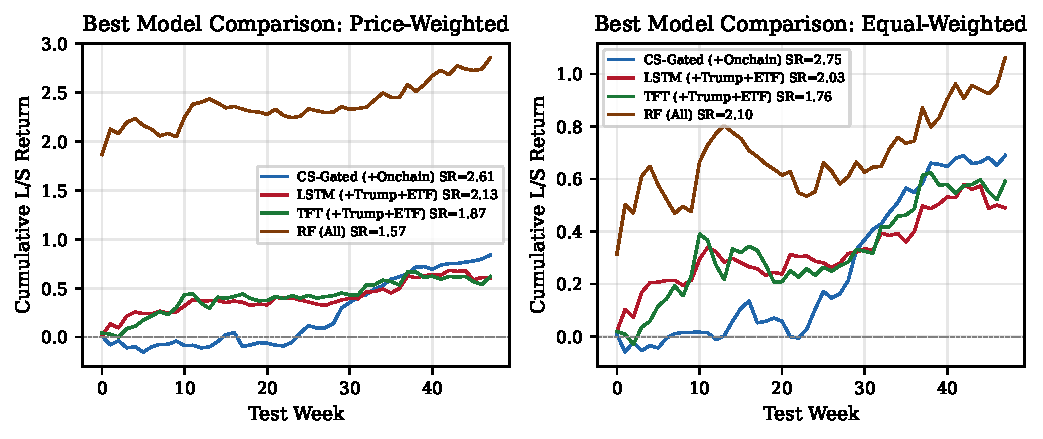
\includegraphics[width=\linewidth]{figures/cum_returns_combined.pdf}
  \caption{Cumulative long-short returns for the best configuration of
           each model (CS-Gated \texttt{+Onchain}, LSTM \texttt{+Trump+ETF},
           TFT \texttt{+Trump+ETF}, and RF \texttt{All}). Legend entries report
           each strategy's terminal cumulative return (CR), i.e.\ the final
           value of the plotted curve; this is a magnitude measure, not the
           risk-adjusted Sharpe ratio of \Cref{fig:sr_combined}.}
  \label{fig:cumret_combined}
\end{figure}

\Cref{fig:cumret_combined} plots the cumulative long-short returns for the
best configuration of the three deep learning models and the best Random
Forest specification.
The figure is broadly consistent with the table-based ranking results:
the strongest specifications separate from zero over the test period, but
they do so through different paths.
RF reaches the largest cumulative level in this figure, especially under
price weighting, but its gains are more episodic and concentrated early in
the test window.
CS-Gated and LSTM accumulate more gradually.
This is consistent with RF's configuration-specific dominance in
\Cref{tab:cross_model} rather than uniform superiority across rows.

%insert Figure — Sharpe ratio comparison
\begin{figure}[t]
  \centering
  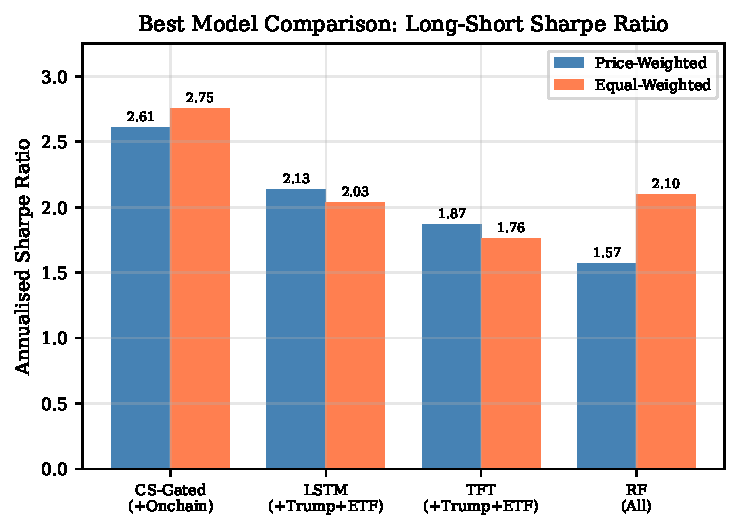
\includegraphics[width=0.8\linewidth]{figures/sr_comparison.pdf}
  \caption{Annualized long-short Sharpe ratios for the best configuration of
           each model (CS-Gated \texttt{+Onchain}, LSTM \texttt{+Trump+ETF},
           TFT \texttt{+Trump+ETF}, and RF \texttt{All}), under price-weighted
           and equal-weighted portfolio construction. Unlike
           \Cref{fig:cumret_combined}, which plots terminal cumulative return,
           this figure reports risk-adjusted performance.}
  \label{fig:sr_combined}
\end{figure}

\Cref{fig:sr_combined} restates the same comparison on a risk-adjusted basis.
CS-Gated (\texttt{+Onchain}) attains the highest Sharpe ratio under both
weighting schemes (2.61 PW, 2.75 EW), whereas Random Forest---despite reaching
the largest cumulative return in \Cref{fig:cumret_combined}---earns the lowest
price-weighted Sharpe ratio (1.57), because its gains are large but volatile.
The two figures therefore measure different objects: cumulative return rewards
total magnitude, while the Sharpe ratio rewards consistency, and it is the
latter that underpins the model ranking in \Cref{tab:cross_model}.

\section{Decile Sharpe Ratios}

\begin{figure}[t]
  \centering
  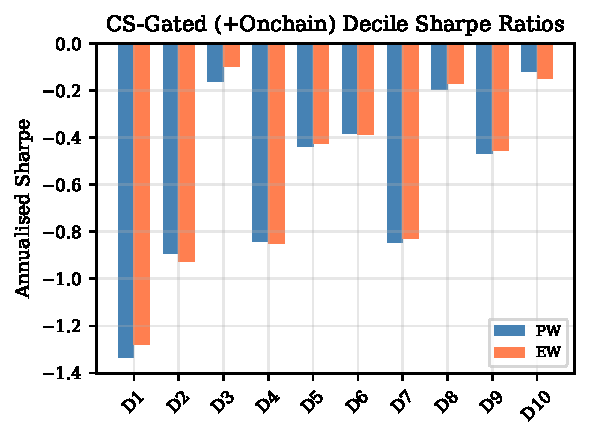
\includegraphics[width=\linewidth]{figures/decile_sharpe_cs_gated.pdf}
  \caption[Decile Sharpe ratios for CS-Gated]{Sharpe ratio of each predicted-rank decile portfolio for
           CS-Gated (\texttt{+Onchain}). Decile 1 corresponds to the
           short leg (lowest predicted rank); decile 10 corresponds to the
           long leg (highest predicted rank). Bars report both PW and EW
           portfolios.}
  \label{fig:decile_cs_gated}
\end{figure}

\Cref{fig:decile_cs_gated} shows the Sharpe ratio of each predicted-rank
decile portfolio for CS-Gated (+Onchain).
The pattern should be interpreted through the long-short spread rather than
as a perfectly monotone decile ladder.
These bars are standalone decile-portfolio Sharpe ratios, whereas
\Cref{tab:cross_model} reports the Sharpe ratio of the D10--D1 long-short
spread; their ordering therefore need not match exactly.
During this test window, several standalone decile portfolios have negative
Sharpe ratios, but the lowest predicted decile performs materially worse than
the highest predicted decile.
The economically relevant result is therefore cross-sectional separation:
the model identifies assets to avoid more strongly than it produces a smooth
ranking across every intermediate bucket.
Middle deciles are noisy, which is unsurprising given only 48 valid weekly
portfolio observations.


\chapter{Analysis}
\label{sec:analysis}
\section{Ablation Study}
\label{sec:analysis:ablation}

To isolate the contribution of the main design choices, we compare three LSTM
variants on the \texttt{Price+Technical} information set:

\begin{enumerate}[label=(\Alph*)]
  \item \textbf{Baseline}: raw-return ListNet targets, no gradient accumulation.
  \item \textbf{+RankNorm}: rank-percentile targets, no gradient accumulation.
  \item \textbf{Full method}: rank-percentile targets with gradient accumulation ($K=4$).
\end{enumerate}

% Auto-generated by gen_tables.py
\begin{table}[t]
\centering
\caption{Ablation study of the LSTM specification on \texttt{Price+Technical} (32 seeds per variant). Ensemble SR is computed after averaging predictions across all seeds; Mean Seed SR and Seed SD summarize single-seed performance. $\Delta$ is the change in Ensemble SR from the preceding specification.}
\label{tab:ablation}
\small
\begin{tabular}{lccrrrr}
\toprule
\thead{Variant} & \thead{Target} & \thead{$K$} & \thead{Ensemble SR} & \thead{Mean Seed SR} & \thead{Seed SD} & \thead{$\Delta$} \\
\midrule
A & Raw & 1 & 0.666 & -0.024 & 0.481 & -- \\
B & Rank pct. & 1 & 0.525 & 0.287 & 0.924 & -0.141 \\
C & Rank pct. & 4 & 1.447 & 0.697 & 0.797 & +0.922 \\
\bottomrule
\end{tabular}
\end{table}


\Cref{tab:ablation} shows that rank normalization by itself does not
automatically raise the ensemble Sharpe ratio: the EW Sharpe moves from
0.666 in Variant A to 0.525 in Variant B.
What rank normalization does achieve is a cleaner and more comparable target
distribution across weeks, reducing the dependence of the loss on raw-return
scale.
This is visible in the single-seed statistics as well:
the mean seed Sharpe improves from $-0.024$ in Variant A to $0.287$ in
Variant B, even though the ensemble result remains weaker.
In other words, the target becomes more informative, but not yet reliably
trainable.
At the same time, the seed standard deviation rises from 0.481 to 0.924,
which indicates that rank normalization alone increases dispersion across
training runs when the effective batch is still too small.
That stabilization becomes economically meaningful only once the effective
batch is enlarged.
From B to C, adding gradient accumulation raises the EW Sharpe to 1.447,
while also lifting the mean seed Sharpe to 0.697 and reducing seed
dispersion to 0.797.
This indicates that the model can exploit the improved target once each
update is based on a richer cross-sectional empirical distribution.

The methodological lesson is straightforward.
The key improvement is not a single architectural tweak, but the combination
of target redesign and training stabilization:
rank normalization aligns the learning target with the cross-sectional
ranking objective, and gradient accumulation makes that objective learnable
in practice.
The full-scale TFT Variable Selection Network is not part of this table,
because it is architecture-specific rather than a shared methodological
component.

\section{Granger Causality of Trump Features}
\label{sec:analysis:granger}

A standard critique of social media predictors is reverse causality:
prices may move first, and posting behavior may simply react to those moves.
To address that concern, we test whether Trump social media features
Granger-cause \citep{granger1969investigating} the cross-sectional mean
return using VAR($p$) models with $p \in \{1,2,4\}$.

% Auto-generated by gen_granger_table.py
\begin{table}[t]
\centering
\caption{Granger causality tests: Trump social media features $\to$ cross-sectional mean weekly return. Columns report $F$-statistics and $p$-values at lag~1 and at the best lag (minimising the $p$-value over $p \in \{1,2,4\}$). VAR($p$) estimated on Trump-period weeks only ($T=112$).}
\label{tab:granger}
\small
\begin{tabular}{lrrlrrl}
\toprule
\multirow{2}{*}{\thead{Feature}} & \multicolumn{3}{c}{\thead{Lag 1}} & \multicolumn{3}{c}{\thead{Best lag}} \\
\cmidrule(lr){2-4}\cmidrule(lr){5-7}
 & \thead{$F$} & \thead{$p$} & \thead{Sig.} & \thead{$F$} & \thead{$p$} & \thead{Lag/Sig.} \\
\midrule
Post count & 1.549 & 0.2159 &  & 1.549 & 0.2159 & lag=1 \\
Caps ratio & 0.002 & 0.9633 &  & 0.104 & 0.9016 & lag=2 \\
Tariff score & 0.021 & 0.8848 &  & 0.911 & 0.4608 & lag=4 \\
Crypto score & 0.222 & 0.6385 &  & 0.627 & 0.5360 & lag=2 \\
Sentiment & 0.003 & 0.9579 &  & 0.517 & 0.5976 & lag=2 \\
\bottomrule
\end{tabular}
\par\vspace{0.35em}
\begin{minipage}{0.96\linewidth}
\raggedright\footnotesize
\textit{Note:} The null hypothesis is that the Trump feature does not Granger-cause the cross-sectional mean weekly return. $^{***}$/$^{**}$/$^{*}$ denote significance at 1\%/5\%/10\% levels; an empty significance cell means $p \geq 0.10$. The best-lag column searches over $\{1,2,4\}$ weekly lags. No multiple-testing adjustment is applied.
\end{minipage}
\end{table}


\Cref{tab:granger} shows that, for the cross-sectional mean weekly return,
none of the five Trump features is statistically significant at conventional
levels under any lag specification.
We therefore cannot claim that Trump posting behavior robustly leads the
market in the time-series mean-return sense.

This result should not, however, be over-interpreted.
The Granger tests are conducted on a single aggregate return series,
whereas our predictive models target the \emph{relative ordering} of tokens
within each week.
A feature may fail to predict whether the market as a whole rises or falls,
yet still help identify which tokens are likely to outperform others.
Moreover, if market reactions occur within the same week as the posts, a
lag-based weekly Granger framework is structurally unlikely to detect them.
The appropriate takeaway is therefore cautious rather than dismissive:
Trump features may be useful as cross-sectional dispersion or narrative
signals, but the evidence does not support a clean claim of market-level
leadership.

\section{Transaction Cost Sensitivity}
\label{sec:analysis:txcost}

Weekly rebalancing of top- and bottom-decile portfolios inevitably introduces
transaction costs, so economic interpretation must go beyond gross Sharpe
ratios.
Using the evaluation logic implemented for the best-performing
CS-Gated \texttt{+Onchain} strategy, turnover is measured from the fraction of
positions that change from one week to the next, with one-way trading costs
applied to both the long and short legs.

% Auto-generated by gen_tables.py -- do not edit manually
\begin{table}[t]
\centering
\caption[Transaction-cost sensitivity]{Transaction-cost sensitivity for the CS-Gated \texttt{+Onchain} equal-weight long-short strategy.}
\label{tab:txcost}
\small
\setlength{\tabcolsep}{4pt}
\begin{tabularx}{\linewidth}{@{}lrrr>{\raggedright\arraybackslash}X@{}}
\toprule
\thead{Scenario} & \thead{Cost} & \thead{Net SR} & \thead{Avg. TO} & \thead{Interpretation} \\
\midrule
Gross & 0 bps & +2.753 & 28.1\% & No trading cost \\
Maker-like & 5 bps & +2.725 & 28.1\% & Low-fee liquid execution \\
Maker-like & 10 bps & +2.697 & 28.1\% & Maker fee plus small spread/slippage \\
Taker-like & 25 bps & +2.614 & 28.1\% & Taker fee or moderate spread \\
Taker-like & 50 bps & +2.475 & 28.1\% & Taker fee plus spread/slippage \\
Stress & 100 bps & +2.198 & 28.1\% & High spread or market-impact allowance \\
Stress & 200 bps & +1.649 & 28.1\% & Severe small-token execution allowance \\
\bottomrule
\end{tabularx}
\par\vspace{0.35em}
\begin{minipage}{0.96\linewidth}
\raggedright\footnotesize
\textit{Note:} Cost is an all-in one-way assumption applied to both long and short legs based on weekly portfolio turnover. Gross EW Sharpe is +2.753; the estimated break-even one-way cost is approximately 510 bps. These scenarios are sensitivity checks, not exchange-specific fee quotes.
\end{minipage}
\end{table}


The purpose of this exercise is not to defend a single exact spread estimate.
Crypto trading costs vary substantially by venue, token liquidity, order type,
and the amount of market impact created by the strategy itself.
Instead, \Cref{tab:txcost} reports a set of transparent one-way cost
assumptions.
The low-cost scenarios correspond to maker-like execution in liquid names,
the middle scenarios approximate taker-like execution, and the high-cost
scenarios add slippage or market-impact allowances.
The results show that the CS-Gated ranking signal is not purely a zero-cost
artifact over this grid, although the table should not be interpreted as a
claim that the strategy is executable at the same cost for every token in the
fixed 86-asset universe.

\section{Sub-Period Robustness}
\label{sec:analysis:subperiod}

Because the test window contains only 49 weeks, aggregate Sharpe ratios may
mask concentration in a single market regime.
We therefore assess robustness across four consecutive sub-periods,
comparing the best CS-Gated specification with the OLS benchmark.

The relevant question is not whether every window produces equally strong
performance, but whether the model remains directionally useful across
different market conditions.
Our evidence indicates that CS-Gated is less dependent on one isolated
episode than OLS, whose performance varies more substantially across windows.
This is consistent with the broader interpretation of the paper: nonlinear
cross-sectional transformations can adapt more flexibly to changing relative
asset structure than fixed linear combinations of characteristics.

\section{TFT Variable Importance}
\label{sec:analysis:importance}

\begin{figure}[t]
  \centering
  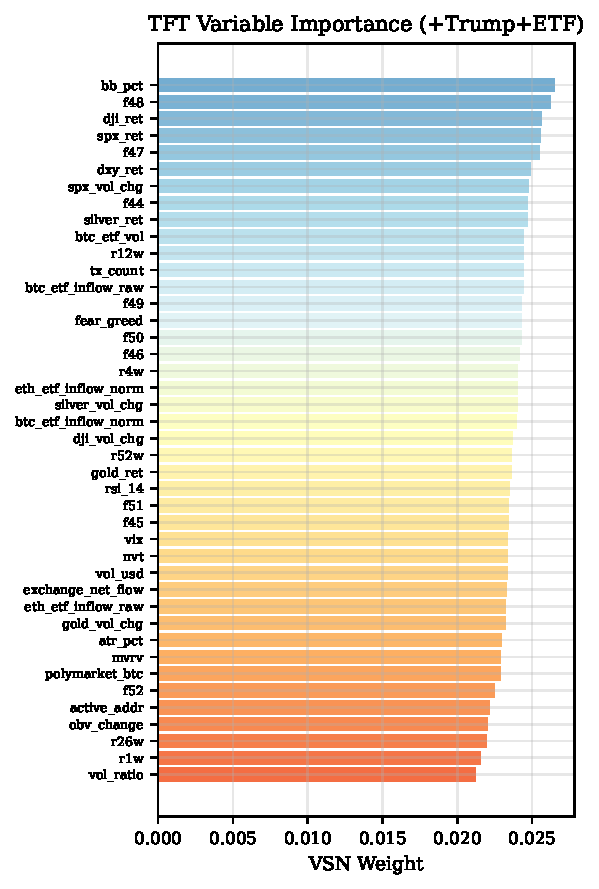
\includegraphics[width=\linewidth]{figures/feat_importance_tft.pdf}
  \caption{TFT Variable Selection Network (VSN) weights for the
           \texttt{+Trump+ETF} configuration, averaged over 32 seeds
           and the test-period observations. Higher weight indicates greater selection
           probability in the VSN softmax.}
  \label{fig:feat_importance}
\end{figure}

TFT provides one of the few architecture-level interpretability mechanisms in
the paper through its Variable Selection Network.
As shown in \Cref{fig:feat_importance}, short-horizon momentum variables
(especially 1-week and 4-week returns) receive the largest average weights,
which is consistent with the role of short-term momentum in cryptocurrency
cross-sections \citep{liu2022cryptocurrency}.
On-chain metrics such as NVT and MVRV occupy an intermediate tier of
importance, suggesting that structural valuation information remains useful
even when richer event-type features are included.

Macro variables receive comparatively lower average weights, indicating that
their effect is more diffuse and indirect.
By contrast, the granular Farside ETF variables receive relatively high
weights despite their shorter sample coverage, which suggests that TFT treats
their non-missing observations as information-dense episodes.
Trump social media features display the highest cross-seed heterogeneity:
some seeds rely on them heavily, others almost ignore them.
This is precisely the kind of instability for which ensembling is valuable,
because averaging allows the final predictor to retain signal that is only
useful intermittently.

\section{Ensemble Size and Per-Seed Variance}
\label{sec:analysis:ensemble}

\Cref{tab:seeds} summarizes per-seed Sharpe ratio statistics for LSTM and TFT.

\begin{table}[t]
\centering
\caption{Per-seed Sharpe ratio statistics (32 seeds, test set, EW).
         Ensemble SR = mean score over 32 seeds; Gain = Ensemble / Per-seed Mean.}
\label{tab:seeds}
\small
\begin{tabular}{llrrrrrr}
\toprule
\thead{Model} & \thead{Config} & \thead{Mean} & \thead{Std} & \thead{Min} & \thead{Max} & \thead{Ensemble} & \thead{Gain} \\
\midrule
LSTM & Price+Tech    & +0.70 & 0.80 & $-$0.77 & +2.51 & +1.45 & 2.1$\times$ \\
LSTM & +Onchain      & +0.41 & 0.75 & $-$1.27 & +1.91 & +1.13 & 2.8$\times$ \\
LSTM & +Trump+ETF    & +0.26 & 0.70 & $-$1.49 & +1.84 & +2.03 & 7.8$\times$ \\
\midrule
TFT  & Price+Tech    & +0.22 & 0.83 & $-$1.11 & +2.18 & +0.12 & 0.5$\times$ \\
TFT  & +Onchain      & +0.49 & 0.71 & $-$1.53 & +1.74 & +1.32 & 2.7$\times$ \\
TFT  & +Trump+ETF    & +0.58 & 0.82 & $-$1.12 & +2.35 & +1.76 & 3.0$\times$ \\
\bottomrule
\end{tabular}
\end{table}

Three points stand out.
First, single deep-learning runs are highly unreliable: per-seed Sharpe ratios
are often mediocre or even negative, despite strong final ensemble
performance.
Second, LSTM benefits more from ensembling than TFT, implying that its seeds
retain greater prediction diversity and therefore offer more scope for noise
cancellation.
Third, this result tempers any simplistic comparison with deterministic
baselines.
Part of deep learning's final advantage in this paper comes from
multi-seed stabilization, not from single-run robustness alone.
That does not invalidate the result, but it does clarify what kind of
“performance” is being claimed: ensemble-level predictive quality rather than
one-shot training reliability.


\chapter{Conclusion}
\label{sec:conclusion}
This paper argues that the central reason deep learning often underperforms in
cross-sectional cryptocurrency prediction is not necessarily architectural
inadequacy, but objective misspecification.
When the task is fundamentally about relative ordering, training on raw-return
targets makes the loss overly sensitive to week-to-week variation in return
scale.
Replacing those targets with rank percentiles, and pairing that change with
gradient accumulation, makes the ranking problem substantially more stable and
translates that stability into out-of-sample performance.

\paragraph{Architecture and signal type.}
The main empirical conclusion is not that one architecture dominates
universally, but that different architectures are well suited to different
signal structures.
CS-Gated performs best when predictive content comes from contemporaneous
on-chain fundamentals, implying that strong cross-sectional structure can be
exploited without explicit temporal encoding.
LSTM and TFT improve materially once Trump social media and granular ETF flow
variables are added, suggesting that temporal architectures are most valuable
when the predictors themselves possess persistence, event clustering, or
sequence-level information.
At the same time, Random Forest remains a powerful benchmark in richer
high-dimensional settings, underscoring that traditional nonlinear methods are
still highly competitive.

\paragraph{Methodological implication.}
The ablation evidence shows that the decisive improvement comes less from a
novel network design than from correcting the supervision signal and making it
trainable.
This has a broader implication for financial machine learning:
reported failures of deep learning may sometimes reflect the fact that models
were optimized against targets misaligned with the actual investment
criterion, rather than the fact that neural architectures are intrinsically
ill-suited to the domain.

\paragraph{Limitations.}
Three limitations remain central.
First, the test period covers only 49 weeks, which constrains statistical
precision.
Second, the 86-asset universe is fixed using March 2026 rankings and therefore
contains survivorship bias.
Third, the strongest deep-learning results rely on multi-seed ensembling, so
their advantage over simpler methods is not the same as single-run
repeatability or computational efficiency.

\paragraph{Future work.}
Several extensions follow naturally from the present results.
The rank-normalized objective could be tested on equity or other
cross-sectional asset universes to assess external validity.
Higher-frequency order-book, microstructure, or narrative-text signals could
be used to identify more precisely which predictors genuinely require temporal
encoding.
Finally, portfolio construction could be extended beyond decile long-short
sorting toward constrained optimization or dynamic position sizing, bringing
the predictive and execution layers of the framework into tighter alignment.


%% ─────────────────────────────────────────────────────────────
%% References
%% ─────────────────────────────────────────────────────────────
\cleardoublepage
\addcontentsline{toc}{chapter}{References}
\renewcommand{\bibname}{References}
\bibliographystyle{plainnat}
\bibliography{references}

%% ─────────────────────────────────────────────────────────────
%% Appendix
%% ─────────────────────────────────────────────────────────────
\appendix
% ============================================================
%  Appendix
% ============================================================

% ─────────────────────────────────────────────────────────────
\chapter{Complete Feature List}
\label{app:features}

Table~\ref{tab:feature_list} lists the 42 features that are actually used in
the six information sets reported in the main text.

\begin{table}[hp]
\centering
\small
\caption{Complete feature list used in the empirical model comparisons,
         with indices, names, and categories.
         $^\dagger$ Newly introduced structural features.}
\label{tab:feature_list}
\begin{tabular}{clll}
\toprule
\thead{Idx} & \thead{Name} & \thead{Category} & \thead{Description} \\
\midrule
0--4   & r1w, r4w, r12w, r26w, r52w & Price Momentum & 1/4/12/26/52-week returns \\
5      & rsi\_14             & Technical       & RSI (14-period) \\
6      & bb\_pct             & Technical       & Bollinger Band \% \\
7      & vol\_ratio          & Technical       & Volume ratio (7-day / 30-day) \\
8      & atr\_pct            & Technical       & ATR as \% of price \\
9      & obv\_change         & Technical       & On-Balance Volume change \\
10     & vol\_usd            & Technical       & USD trading volume \\
11     & active\_addr        & On-chain        & Active addresses \\
12     & tx\_count           & On-chain        & Transaction count \\
13     & nvt                 & On-chain        & Network Value to Transactions \\
14     & exchange\_net\_flow & On-chain        & Exchange net flow \\
15     & mvrv                & On-chain        & Market Value / Realized Value \\
16     & fear\_greed         & Macro/Sentiment & Crypto Fear \& Greed Index \\
17     & spx\_ret            & Macro           & S\&P 500 weekly return \\
18     & dxy\_ret            & Macro           & DXY (USD Index) return \\
19     & vix                 & Macro           & VIX volatility index \\
20     & gold\_ret           & Macro           & Gold return \\
21     & silver\_ret         & Macro           & Silver return \\
22     & dji\_ret            & Macro           & Dow Jones return \\
23     & spx\_vol\_chg       & Macro           & S\&P 500 vol change \\
24     & gold\_vol\_chg      & Macro           & Gold vol change \\
25     & silver\_vol\_chg    & Macro           & Silver vol change \\
26     & dji\_vol\_chg       & Macro           & DJI vol change \\
27     & btc\_etf\_inflow\_norm  & ETF/Prediction & BTC ETF inflow (normalized) \\
28     & polymarket\_btc         & ETF/Prediction & Prediction-market BTC probability \\
29     & btc\_etf\_inflow\_raw   & ETF/Prediction & BTC ETF inflow (raw) \\
30     & eth\_etf\_inflow\_norm  & ETF/Prediction & ETH ETF inflow (normalized) \\
31     & eth\_etf\_inflow\_raw   & ETF/Prediction & ETH ETF inflow (raw) \\
32     & btc\_etf\_vol           & ETF/Prediction & BTC ETF volume \\
44     & trump\_post\_count      & Trump Social   & Weekly post count \\
45     & trump\_caps\_ratio      & Trump Social   & Caps ratio (intensity) \\
46     & trump\_tariff\_score    & Trump Social   & Tariff/trade post fraction \\
47     & trump\_crypto\_score    & Trump Social   & Crypto post fraction \\
48     & trump\_sentiment        & Trump Social   & Exclamation density \\
49$^\dagger$ & btc\_etf\_gbtc       & Farside ETF & GBTC weekly net flow (\$M) \\
50$^\dagger$ & btc\_etf\_excl\_gbtc & Farside ETF & BTC ETF ex-GBTC net flow \\
51$^\dagger$ & eth\_etf\_ethe       & Farside ETF & ETHE weekly net flow (\$M) \\
52$^\dagger$ & eth\_etf\_excl\_ethe & Farside ETF & ETH ETF ex-ETHE net flow \\
\bottomrule
\end{tabular}
\end{table}

% ─────────────────────────────────────────────────────────────
\chapter{Model Parameter Counts}
\label{app:params}

\begin{table}[h]
\centering
\small
\caption{Approximate parameter counts per model
         (hidden\_dim=64, 2 heads, 1 LSTM layer).
         Parameter count varies with $M$ only in the input projection layer.}
\label{tab:params}
\begin{tabular}{lrr}
\toprule
\thead{Model} & \thead{Params (approx.)} & \thead{vs.\ Baseline} \\
\midrule
CS-Gated (Proposed) & 49--75K        & N/A \\
LSTM                & $\sim$53K      & $-36\%$ (Baseline: 82K) \\
TFT                 & $\sim$90--100K & $-75\%$ (Baseline: 368K) \\
\midrule
Random Forest     & N/A (300 trees) & --- \\
Gradient Boosting & N/A             & --- \\
OLS               & $M+1$ (linear)  & --- \\
\bottomrule
\end{tabular}
\end{table}

% ─────────────────────────────────────────────────────────────
\chapter{Per-Seed SR Statistics (Full Table)}
\label{app:seeds}

\begin{table}[h]
\centering
\small
\caption{Per-seed Sharpe ratio statistics across all feature configurations
         (32 seeds, price-weighted long-short, test set).
         Ensemble SR = mean prediction over 32 seeds.}
\label{tab:seeds_full}
\begin{tabular}{llrrrrr}
\toprule
\thead{Model} & \thead{Config} & \thead{Mean} & \thead{Std} & \thead{Min} & \thead{Max} & \thead{Ensemble} \\
\midrule
LSTM & Price+Technical & $+$0.70 & 0.80 & $-$0.78 & $+$2.51 & $+$2.46 \\
LSTM & +Onchain        & $+$0.41 & 0.75 & $-$1.27 & $+$1.91 & $+$0.93 \\
LSTM & All             & $+$0.48 & 0.82 & $-$1.51 & $+$2.38 & $+$0.59 \\
LSTM & +Trump          & $+$0.63 & 0.83 & $-$1.16 & $+$2.21 & $+$0.57 \\
LSTM & +ETF            & $+$0.46 & 0.99 & $-$1.54 & $+$2.48 & $+$0.35 \\
LSTM & +Trump+ETF      & $+$0.26 & 0.70 & $-$1.49 & $+$1.84 & $+$2.13 \\
\midrule
TFT  & Price+Technical & $+$0.24 & 0.84 & $-$1.11 & $+$2.18 & $+$0.19 \\
TFT  & +Onchain        & $+$0.51 & 0.71 & $-$1.53 & $+$1.72 & $+$1.30 \\
TFT  & All             & $+$0.51 & 0.83 & $-$1.52 & $+$1.82 & $+$0.17 \\
TFT  & +Trump          & $+$0.47 & 0.85 & $-$1.11 & $+$2.71 & $+$0.98 \\
TFT  & +ETF            & $+$0.65 & 0.76 & $-$0.73 & $+$2.07 & $+$0.87 \\
TFT  & +Trump+ETF      & $+$0.57 & 0.82 & $-$1.12 & $+$2.35 & $+$1.89 \\
\bottomrule
\end{tabular}
\end{table}

% ─────────────────────────────────────────────────────────────
\chapter{Feature Configuration Sizes}
\label{app:configs}

\begin{table}[h]
\centering
\small
\caption{Feature index ranges for each information set.}
\label{tab:configs}
\begin{tabular}{lrl}
\toprule
\thead{Configuration} & \thead{$M$} & \thead{Feature Indices} \\
\midrule
Price+Technical & 11 & 0--10 \\
+Onchain        & 16 & 0--15 \\
All             & 33 & 0--32 \\
+Trump          & 38 & 0--32, 44--48 \\
+ETF            & 37 & 0--32, 49--52 \\
+Trump+ETF      & 42 & 0--32, 44--48, 49--52 \\
\bottomrule
\end{tabular}
\end{table}


\end{document}
